\chapter{Implementation}
\label{cpt:Implementation}

In this chapter, a practical implementation of a consensus-inspired redundant architecture is presented.
The sources are publicly available on GitHub~\cite{GitHubSources}.
The applied consensus algorithm is based on the concepts of \texttt{Raft}.
This implementation's aim is to showcase the practicability and performance of a redundant architecture that applies \abr{DCPS} concepts for finding a consensus in an \abr{ETCS} context, even in the presence of individual component failures.
\\

At first in this chapter, the structure of the implemented system is presented.
Therefore, the utilized hardware, the network topology, and the software structure are described.
In the second section, the way the system manages its state is explained.
Afterward, the system's behavior is outlined in two steps.
First, a leader election algorithm - the basis for further processing - is shown.
Second, the decision-making algorithm, which is based on redundant computation and majority voting, is presented.
Finally in this chapter, methods for system recovery are described.
These include an active hardware redundancy approach as well as a hardware watchdog.

\section{System Structure}

\begin{figure}[!ht]
	\centering
	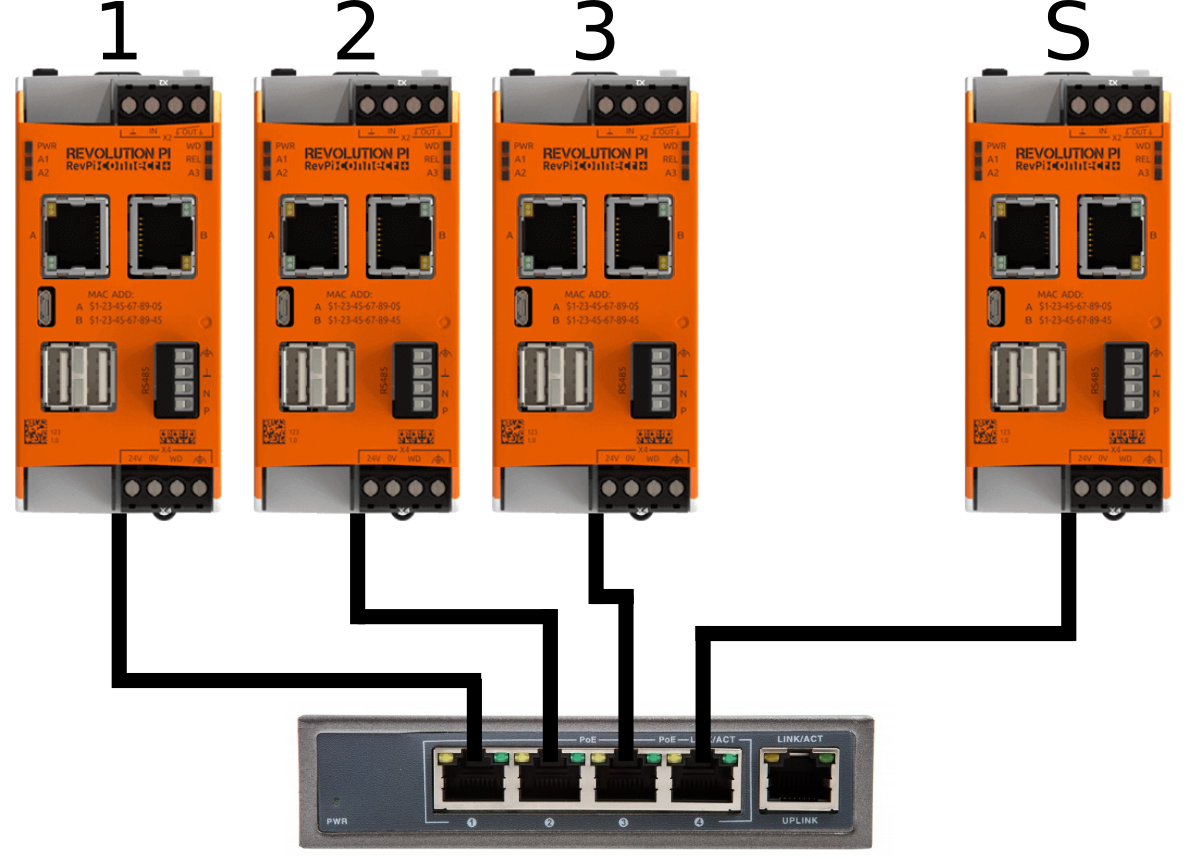
\includegraphics[width=0.8\linewidth]{images/setup}
	\caption{Three homogeneous \textit{Revolution Pi Connects} make up the redundant system which is implemented in the course of this thesis. The replicas are interconnected via a network switch. A fourth \textit{Revolution Pi Connect} acts as a spare unit that is activated upon a failure of any other replica.}
	\label{fig:SystemSetup}
\end{figure}

\begin{figure}[!hb]
	\centering
	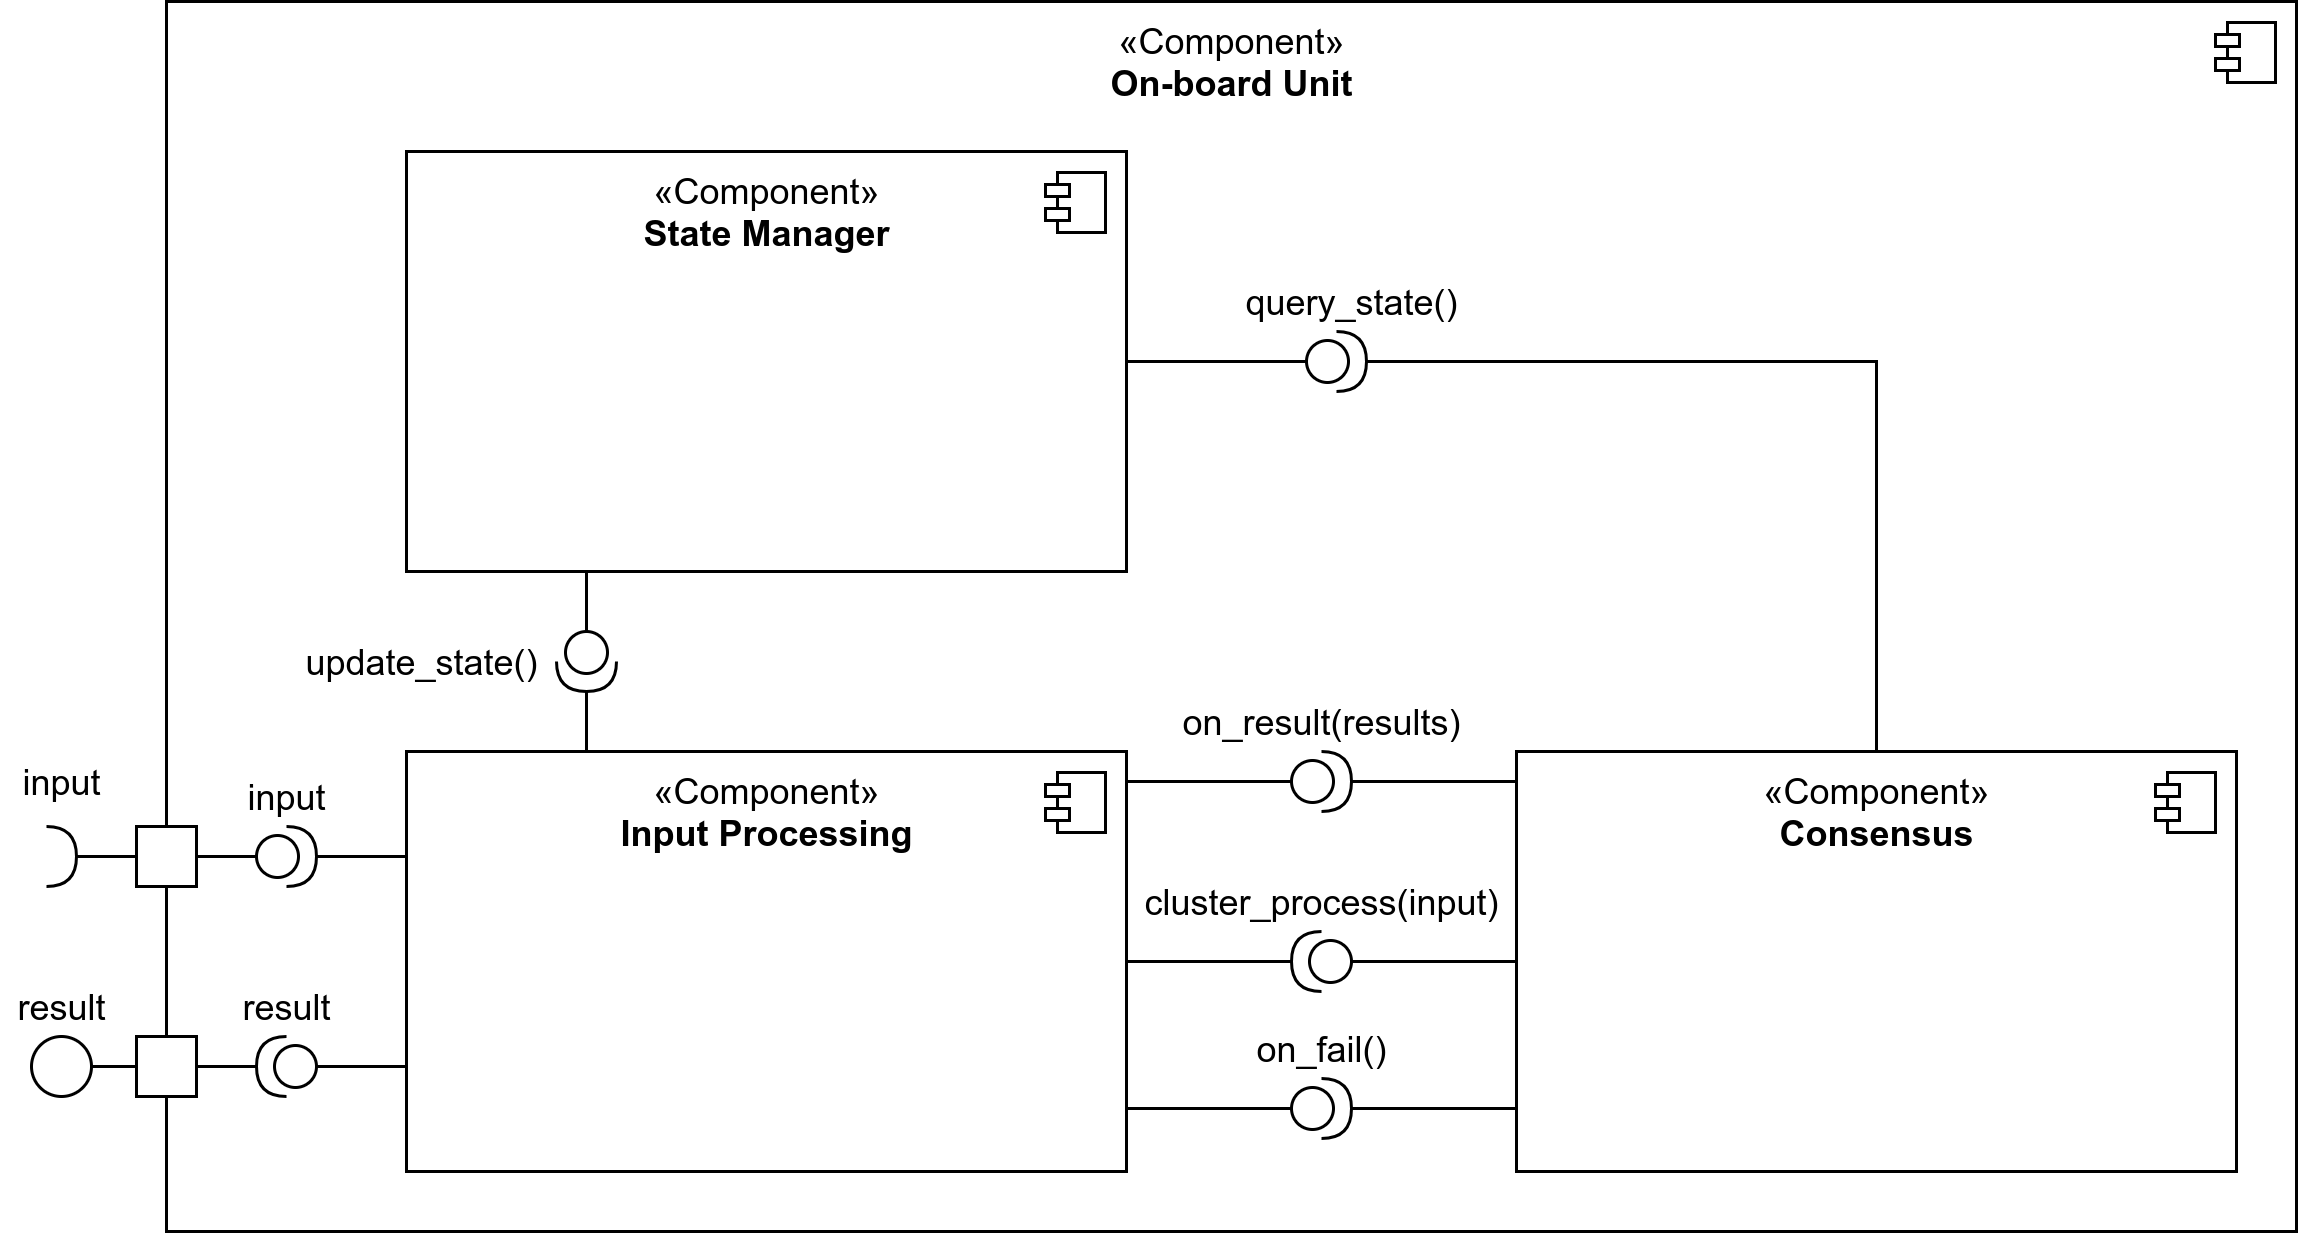
\includegraphics[width=0.9\linewidth]{images/Components}
	\caption{The on-board unit's program, which runs on each replica, consists of three major components. The \texttt{input processing} component reads inputs and performs the voting. While the \texttt{state manager} component administers the system's global state, the \texttt{consensus} component ensures that a leader is present in the system and provides an interface to perform redundant processing.}
	\label{fig:SystemComponents}
\end{figure}

The system's setup to implement the architecture from~\autoref{fig:ThreeRepConsensusDDS} is depicted in~\autoref{fig:SystemSetup}.
Four homogeneous replicas are interconnected via a network switch.
While three replicas are operating in a \abr{TMR} setup, the fourth is used as a spare unit that can be activated on demand, for example when another replica failed.
Each replica is represented by a \textit{Revolution Pi Connect}, an open-source \abr{PLC} that builds upon a Raspberry Pi and is developed by \texttt{Kunbus}.
As such, it features a Broadcom BCM2837 quad-core ARM Cortex A53 1.2 GHz \abr{CPU} and 1 GB \abr{RAM}.
The used \abr{OS} is an extended \textit{Raspbian} \abr{OS} that has been patched with real-time support.
The solution is implemented in the C-programming language and makes use of the C \abr{API} of \textit{Votex OpenSplice DDS} by \texttt{ADLINK}.
\\

A general outline of the system's structure is provided in~\autoref{fig:SystemComponents}.
The \texttt{Input Processing} component provides an interface to the system's environment.
Information about \abrpl{MA}, linked balises, and balise telegrams can be transferred to the system via the \textit{input} interface.
Via the \textit{result} interface, the votet result for a corresponding input is presented.
\\

The system distinguishes between two message types; informative and critical messages.
Informative messages, such as a \abr{MA} or a set of linked balises, alter the system's state.
Upon receiving an informative message, the system's leader integrates the information into the system's global state by utilizing the \texttt{State Manager} component's \textit{update\_state()} functionality.
Critical messages, such as balise telegrams, require the system to make a decision.
After receiving a critical message, the system's leader applies the \texttt{Consensus} component to generate a system-wide decision.
Every replica generates a decision based on the system's global state.
When the decision-making succeeded, the \textit{on\_result} callback is called.
Otherwise, \textit{on\_fail} would be invoked.
\\

Because the network is arranged in a star network, the network switch makes up a single point of failure.
For safety-reasons, a fully connected network would be the better choice.
However, since the software implementation is independent of the applied network topology, a star network was chosen due to cost reasons.

The communication channel is implemented via \textit{Ethernet} and no information redundant communication channel is applied in this demonstration.
Further, no N-version programming is applied, which means that each replica runs the same software implementation.
In order to build a highly secure system, the mentioned compromises need to be further addressed.

\section{System State}
\label{sec:stateManager}
It is mandatory for the replicas in the distributed system to produce deterministic results and to have access to the most recent global system state.
The system's state is stored as a global state in \abr{DDS} state topics and consequently managed by the middleware.
This ensures that all replicas can operate on the most recent system state and no replica becomes outdated.
Only the system's leader is permitted to alter the system's state, all other replicas have read-only access.
Three \abr{DDS} state topics make up the global system state.
\\

The currently valid \abr{MA} is stored in the \texttt{MovementAuthority} topic.
A \abr{MA} is transmitted to the system before a journey starts and is valid for an entire journey.
Hence, a \abr{MA} is stored in an enduring state topic (ref.~\autoref{tab:stateQOS}) so that it is reliably transmitted to all replicas.
Further, the currently valid \abr{MA} is transmitted to late joining replicas.

The set of linked balises is managed by the \texttt{LinkedBalises} topic.
As for \abrpl{MA}, a set of linked balises is assigned once and is valid for an entire journey so that an enduring state topic is used.
Further, because multiple balise instances are managed via this topic, an unique identifier is used to distinguish the balises.

The train's position and speed are stored in the \texttt{TrainState} topic.
Three variables are used for the position.
One encodes the estimated position and two delimit an interval - the so-called confidence interval - that contains the train's actual position.
The topic further contains information about whether the train is moving.
Because the state data is updated periodically and frequently, it is managed as a volatile \abr{DDS} state topic.
\\

The different state topic's data is read and written like any other \abr{DDS} topic.
However, before starting a new journey, it is mandatory to ensure that any information about previous \abrpl{MA} and linked balises is no longer accessible.
In order to circumvent this situation beforehand, any data on the \texttt{MovementAuthority} and \texttt{LinkedBalises} topic is disposed before new data is written.

\section{System Behaviour}

In this section, the components used for processing inputs are described.
The basis for further processing is the election of a system leader.
Upon receiving a critical input, a system-wide decision is made based on redundant computation.
Therefore, a leader election algorithm that applies a \abr{DCPS} communication pattern and follows the concepts of \texttt{Raft} is presented.
Afterward, an algorithm for creating a voted decision based on redundant results is presented.
For both algorithms, safety and timing considerations are described.
\\

For the application to notice that data samples are available on topics, \abr{DDS} \texttt{WaitSets} are used.
\texttt{WaitSets} are preferred over \abr{DDS} \texttt{Listeners} because they are state-based rather than event-based, which means they trigger as long as the system is in a specific state rather than when an event is triggered.
Thereby, \texttt{WaitSets} ensure that no available data is missed.
Further, by using \texttt{WaitSets}, complete control over the application logic is managed by the application itself.
If \texttt{Listeners} had been used, the application logic that should be executed upon the event would be managed by the middleware.
As a result, the application logic cannot block the middleware when using \texttt{WaitSets}.
\\

As depicted in~\autoref{fig:ThreeRepConsensusDDS}, the replicas are communicating via \abrpl{RPC} that are represented by \abr{DDS} event topics.
Although only one topic has been considered for each \abr{RPC} so far, a distinct \abr{DDS} topic for requesting and answering to \abrpl{RPC} is required in practice.
This is because topics in \abr{DDS} need to be in a particular data format.
Thus, an event topic called \texttt{AppendEntriesReply} is used to answer to messages send via \texttt{AppendEntries}.
The same applies for \texttt{RequestVote}, whose response topic is \texttt{RequestVoteReply}.


\subsection{Leader Election}
\begin{figure}[!hb]
	\centering
	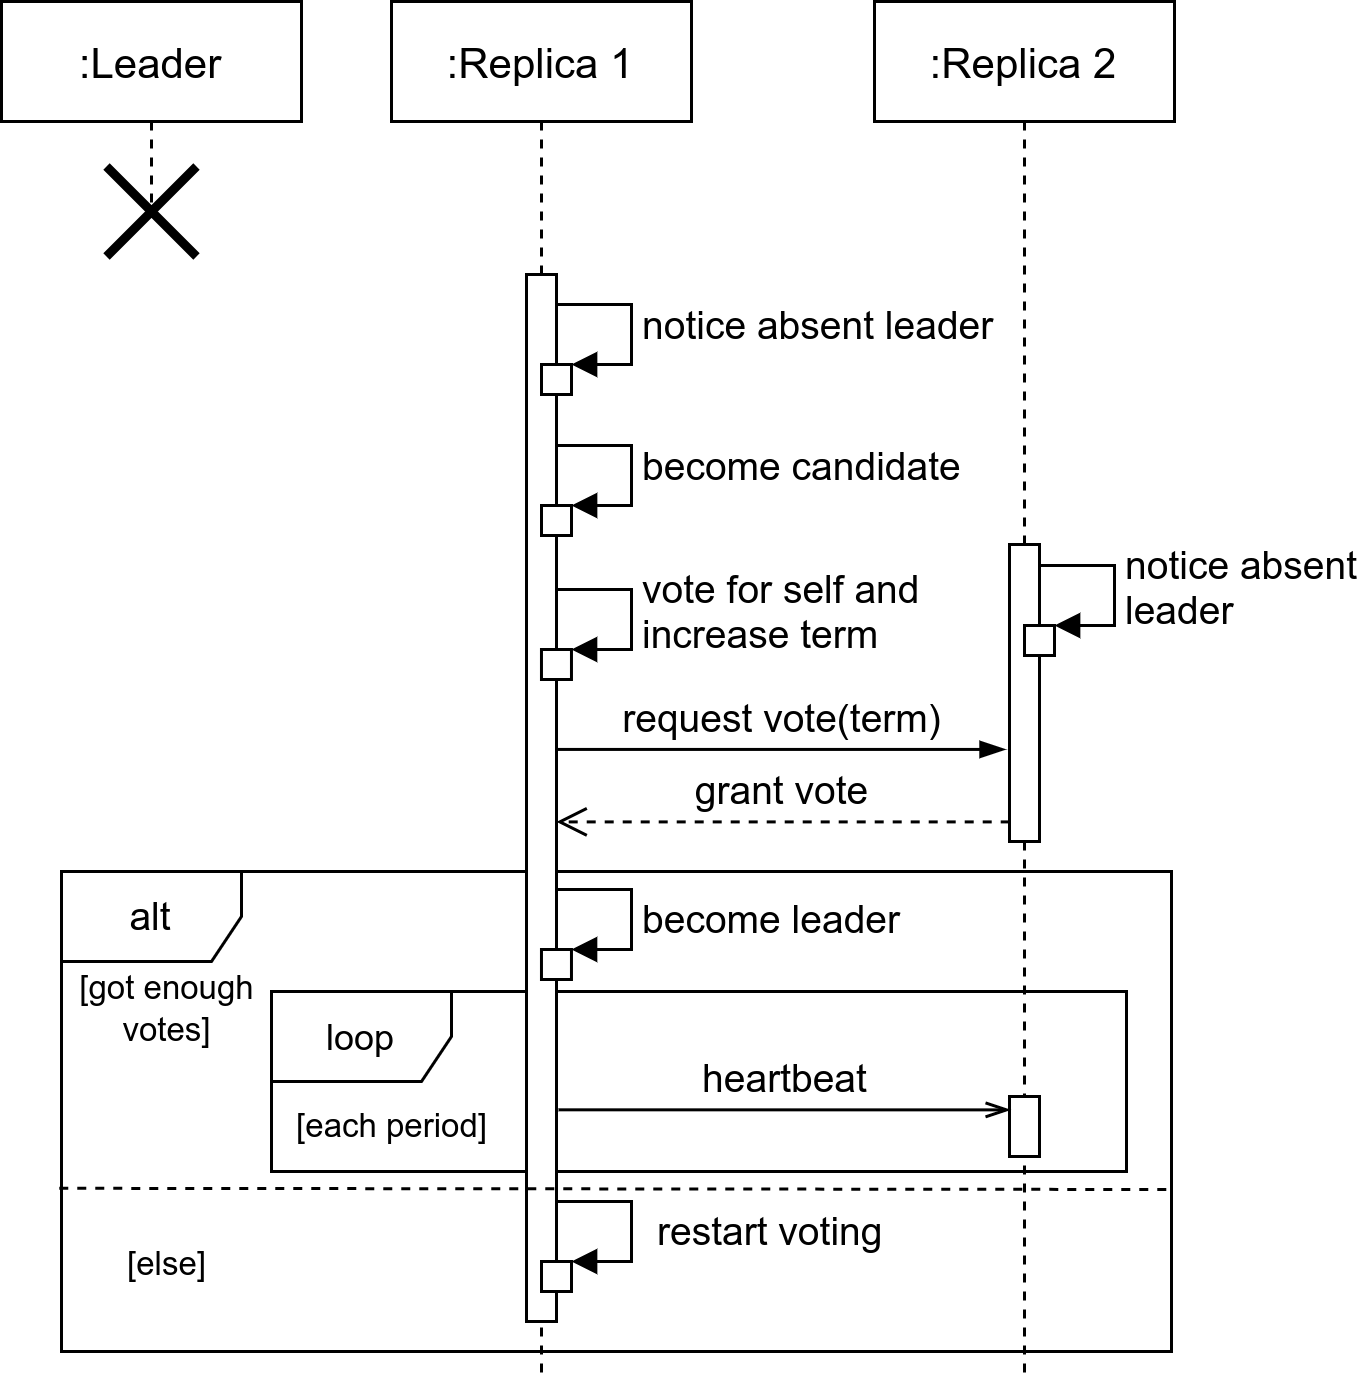
\includegraphics[width=0.75\linewidth]{images/sequence/LeaderElection}
	\caption{When a replica notices that the leader crashed, it becomes a candidate, votes for itself and sends vote requests to all remaining replicas. When enough votes are granted, it becomes the new leader and starts sending heartbeats. Otherwise, it retries to become the leader in the next term.}
	\label{fig:SeqLeaderElection}
\end{figure}

A consensus algorithm guarantees that there is at most one leader present in the system at a time and that a new leader is elected when there is none present.
The remaining replicas transition to follower mode when they recognize a leader.
Time in \texttt{Raft} is subdivided into \textit{terms}, that each start with a leader election.
When a follower recognizes a missing leader in the system, it starts a new term and promotes to become the new leader. 
Each replica manages its term, its current role, and voting information as a private replica state.
\\

It is the leader's responsibility to inform the remaining replicas about its existence.
Therefore, the leader periodically publishes heartbeat messages onto the \texttt{AppendEntries} topic.
When a replica does not receive a message from a leader for a specific period of time, called the \textit{election timeout}, it promotes to become the new leader.
A high-level overview of a voting process is depicted in~\autoref{fig:SeqLeaderElection}.
Replica \textbf{1} notices the crashed leader first and promotes to become the new leader by switching into candidate mode and sending a vote request to each remaining replica.
In the exemplary case in~\autoref{fig:SeqLeaderElection}, replica \textbf{2} accepts the vote request and replica \textbf{1} becomes the new leader.
It immediately starts sending heartbeat messages afterwards.
\\
In the following, the allocation and the collection of votes will be discussed in more detail.
\\\\

\begin{algorithm}[H]
\caption{Algorithm for vote allocation. Whether a vote gets granted or rejected depends on whether the replica that receives the vote request has already voted for another replica in the voting term.}\label{algo:VoteAllocation}
\SetKwData{Term}{\textit{term}}
\SetKwData{Sender}{\textit{senderID}}
\SetKwInOut{Input}{input}
\SetKwInOut{Output}{output}

\Input{A vote request with a \Term and a \Sender}
\Output{true if the vote for \Sender in \Term was granted, false otherwise}
\BlankLine
\If{\Term $>$ current term}{become follower in new \Term\;}
\If{\Term $==$ current term \textbf{AND} not voted in current term}{grant vote for \Sender\;}
\end{algorithm}

The allocation of votes is shown in~\autoref{algo:VoteAllocation}.
Each replica can only vote for one other replica in every term.
Because the system's state is managed globally by \abr{DDS}, every replica is equally up to date so that vote allocation only depends on the promoting replica's term.
As soon as a vote request is received that has a higher term number than the receiving replica's term, the replica automatically transitions into follower mode.
Afterward, it grants the vote for the promoting replica.
Only a single leader is allowed to be active in a term so that replicas are not allowed to vote for multiple replicas in a single term.
\\

\begin{algorithm}[H]\caption{Algorithm for vote collection. Only votes that were answered in the same term that the vote request was issued are considered. When enough votes are collected, the replica becomes the leader. If a vote was answered in a more recent term, the vote collection is aborted and the replica becomes a follower.}\label{algo:VoteCollection}
\SetKwData{VoteTerm}{\textit{voteTerm}}
\SetKwData{VoteGranted}{\textit{voteGranted}}
\SetKwInOut{Input}{input}
\SetKwInOut{Output}{output}

\Input{A vote reply with a \VoteTerm and a \VoteGranted flag}
\Output{Transition to either leader or follower state}
\BlankLine

\If{the replica is no candidate anymore}{return\;}
\If{\VoteTerm $>$ term when election started}{
become follower\;
return\;}
\If{\VoteTerm $==$ term when election started \textbf{AND} vote got granted}{
Increase number of granted votes in the election term\;
	\If{got enough votes}{
	become leader\;
	return\;}
}
\end{algorithm}

Whether a promoting replica becomes the new leader depends on the number of accepted vote requests.
For each received vote reply, the promoting replica first checks whether it has left the candidate state in the meantime, which makes the entire vote reply irrelevant.
This can, for example, happen when another vote request with a higher term number has been granted while the replica itself waits for incoming vote replies.
Afterward, it is checked whether the term of the processing replica was higher than the term in which the voting was started.
This fact indicates that the promoting replica is outdated, so that it should not become a leader and transition into follower mode.
Finally, when the vote got granted and enough granted votes were received, the replica is elected as a new leader for the corresponding term.
The number of necessary voted depends on the total number of replicas in the system and is specified in advance.

\begin{figure}[!hb]
	\centering
	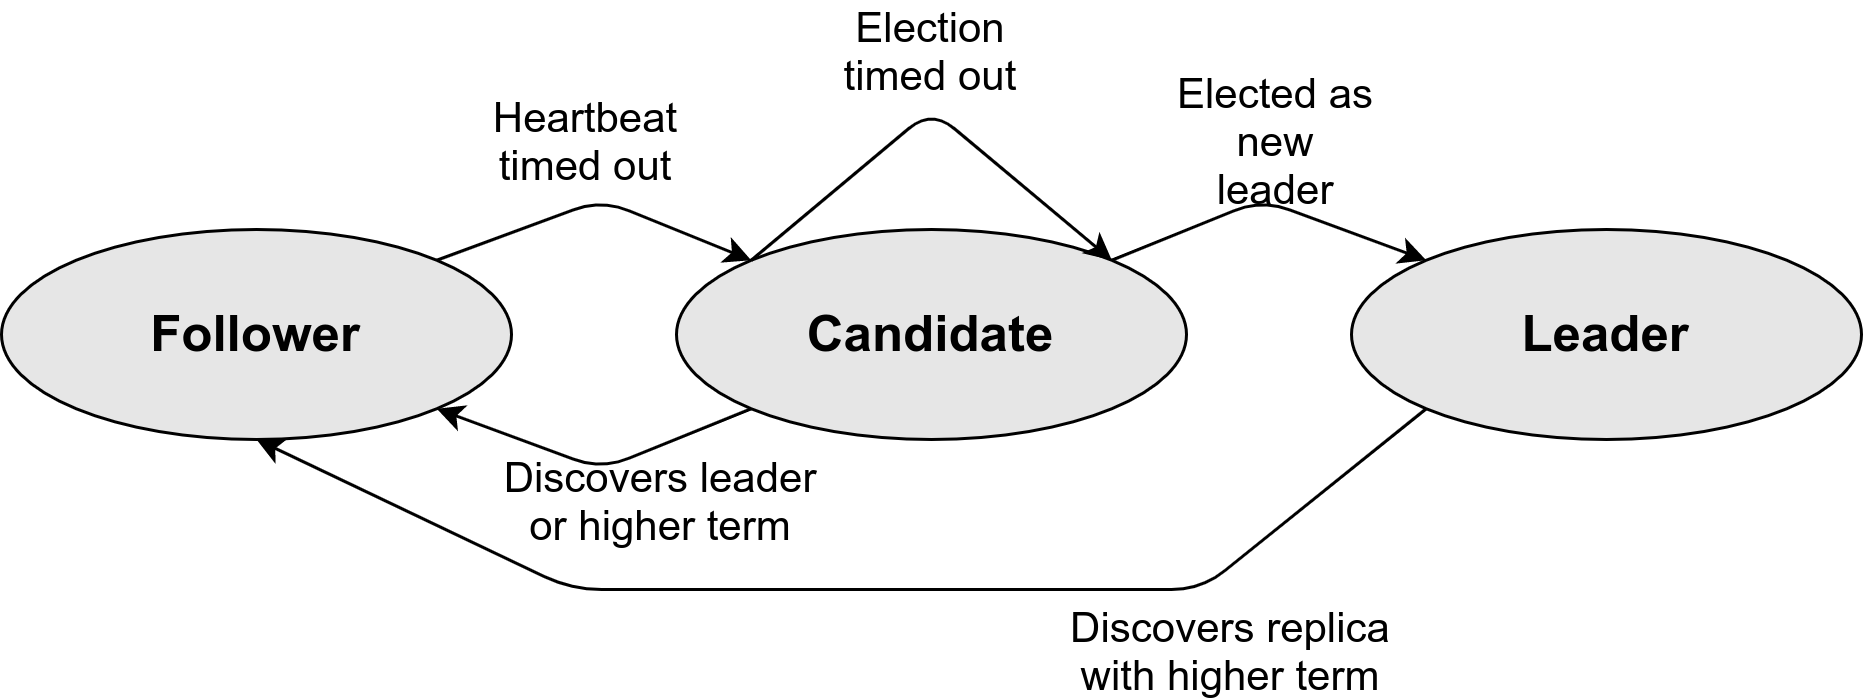
\includegraphics[width=0.75\linewidth]{images/RaftServerStates}
	\caption{Replicas in \texttt{Raft} can be in one of three states. When a follower receives no heartbeat messages from a leader, it starts an election and tries to become the new leader. A replica remains in the candidate state either until it becames the new leader or until it receives a heartbeat from another leader with a higher term. Leaders operate until they fail or until they discover that their term is outdated. This diagram was taken from~\cite{RaftConsensusPaper}}
	\label{fig:RaftServerStates}
\end{figure}


\subsubsection{Safety Considerations}
\label{subsub:raceConditions}

It is crucial for the system's safety that only one leader is present at any time.
Further, it needs to be ensured that a new leader is elected after the previous leader failed and that the system is not without a leader for too long.
When a leader election is impossible, the remaining replicas must ensure that the train stops.
This can lead to situations where multiple replicas at once take control about the system's output.
Therefore, only the most restrictive output should be taken - in this case stopping the train.
Specialized multiplexing hardware that filters simultaneous outputs can ensure that always the most restrictive output is taken.
Other hardware, such as gravity-controlled switches, can ensure that a train stops when no replica is active at all.
\\

The election algorithm is implemented as a concurrent algorithm.
Because no assumptions about the thread's relative speed can be made, race conditions can occur~\cite{Dijkstra1965}.
In the following, it is described how the algorithm ensures functional correntness with \abr{DDS} features and prevents race conditions.

\paragraph{Functional Correctness}
During the entire time, each replica is in one of three states, namely \texttt{Leader}, \texttt{Candidate} or \texttt{Follower}.
The leader election process can be summarized as transitions and corresponding conditions between these three states, as depicted in~\autoref{fig:RaftServerStates}.
Five requirements can be derived from the figure that must be met by an algorithm that implements \texttt{Raft}'s leader election process:

\begin{enumerate}
\item \textbf{Start Election:} A follower becomes a candidate, increments its term, votes for itself, and sends a message to all other replicas stating that it wants to become the leader.
\item \textbf{End of Election:} A candidate remains in candidate state until it either wins the election, receives information about another leader in the system, or times out.
\item \textbf{Won Election:} A candidate wins the election if it receives votes from a majority of replicas in the same term. Each replica votes for at most one replica in a given term.
\item \textbf{Lost Election:} A candidate loses the election when it receives a message from a leader whose term is at least as high as the candidate's term.
\item \textbf{No Result:} A certain period of time goes by without the candidate winning or loosing the election.
\end{enumerate}

For realizing the leader election algorithm with \abr{DCPS} features, three \texttt{Topics} are required.
The \texttt{AppendEntries} and \texttt{RequestVote} topics are representatives for the corresponding \texttt{Raft} \abrpl{RPC}.
Because data objects managed by \abr{DDS} require a predetermined structure, a dedicated topic for replying to vote requests is required.
Therefore, \texttt{RequestVoteReply} is utilized.

A missing leader is detected by not receiving heartbeat messages for a certain period of time.
This period of time is called \textit{election timeout}.
For implementing an \textit{election timeout}, a \texttt{WaitSet} with a corresponding \texttt{ReadCondition}, that triggers when new data has been published to \texttt{AppendEntries}, is applied.
Further, a timeout is attached to the \texttt{WaitSet} that matches the \textit{election timeout}.
This way, if no heartbeat message is received for the \textit{election timeout} period, an event is triggered.
Although a heartbeat message is a periodic message and a deadline \abr{QOS} could be used to register an absent leader, a timeout is preferred.
This is because a \texttt{WaitSet} with a timeout is required for other messages as well and the deadline \abr{QOS} would require a \texttt{StatusCondition} to be noticed whereby the utilized \abr{DDS} subset would grow.
In order to initiate the voting process, the replica publishes a new vote request to \texttt{RequestVote}.
Because the middleware ensures that data is transmitted to all replicas that subscribed to a topic, the \textbf{Start Election} requirement can easily be solved with \abr{DDS}.
\\

Further, \textbf{No Result} can be resolved by using a \texttt{WaitSet}, called \textit{leaderElection\_WaitSet}, with a corresponding timeout (\textit{leader ready timeout}).
When the timeout expires, the replica starts to wait for heartbeat messages again.
In addition to the timeout, a \texttt{ReadCondition} is attached to the \textit{leaderElection\_WaitSet} that triggers when messages from a leader have been published to the \texttt{AppendEntries} topic.
Thereby, \textbf{Lost Election} is ensured.
By implication, this means that the candidate either won the election for the term, or the election was not successful.
An election was unsuccessful when the timeout attached to \textit{leaderElection\_WaitSet} expires.
Thus, \textbf{Won Election} is partly solved.

In order to fully solve \textbf{Won Election}, each replica needs to collect votes and reply to vote requests, parallel to detecting other leaders and voting timeouts.
The voting part is therefore treated by another \abr{OS} thread, that again makes use of a \texttt{WaitSet}, where two \texttt{QueryConditions} are attached to, one for the \texttt{RequestVote} and one for the \texttt{RequestVoteReply} topic.
Thereby, the replicas can agree to a vote request while the candidate waits for the voting to end.

In the case of a network partition, where one or multiple replicas are separated from the others, split-brain situations with multiple leaders - one for each subnet - could happen.
However, the quorum required for voting prevents multiple replicas in a partitioned network to become the leader and prevent split-brain situations from leading to system failures.

\paragraph{Absence of Race Conditions}

\begin{figure}[!ht]
	\centering
	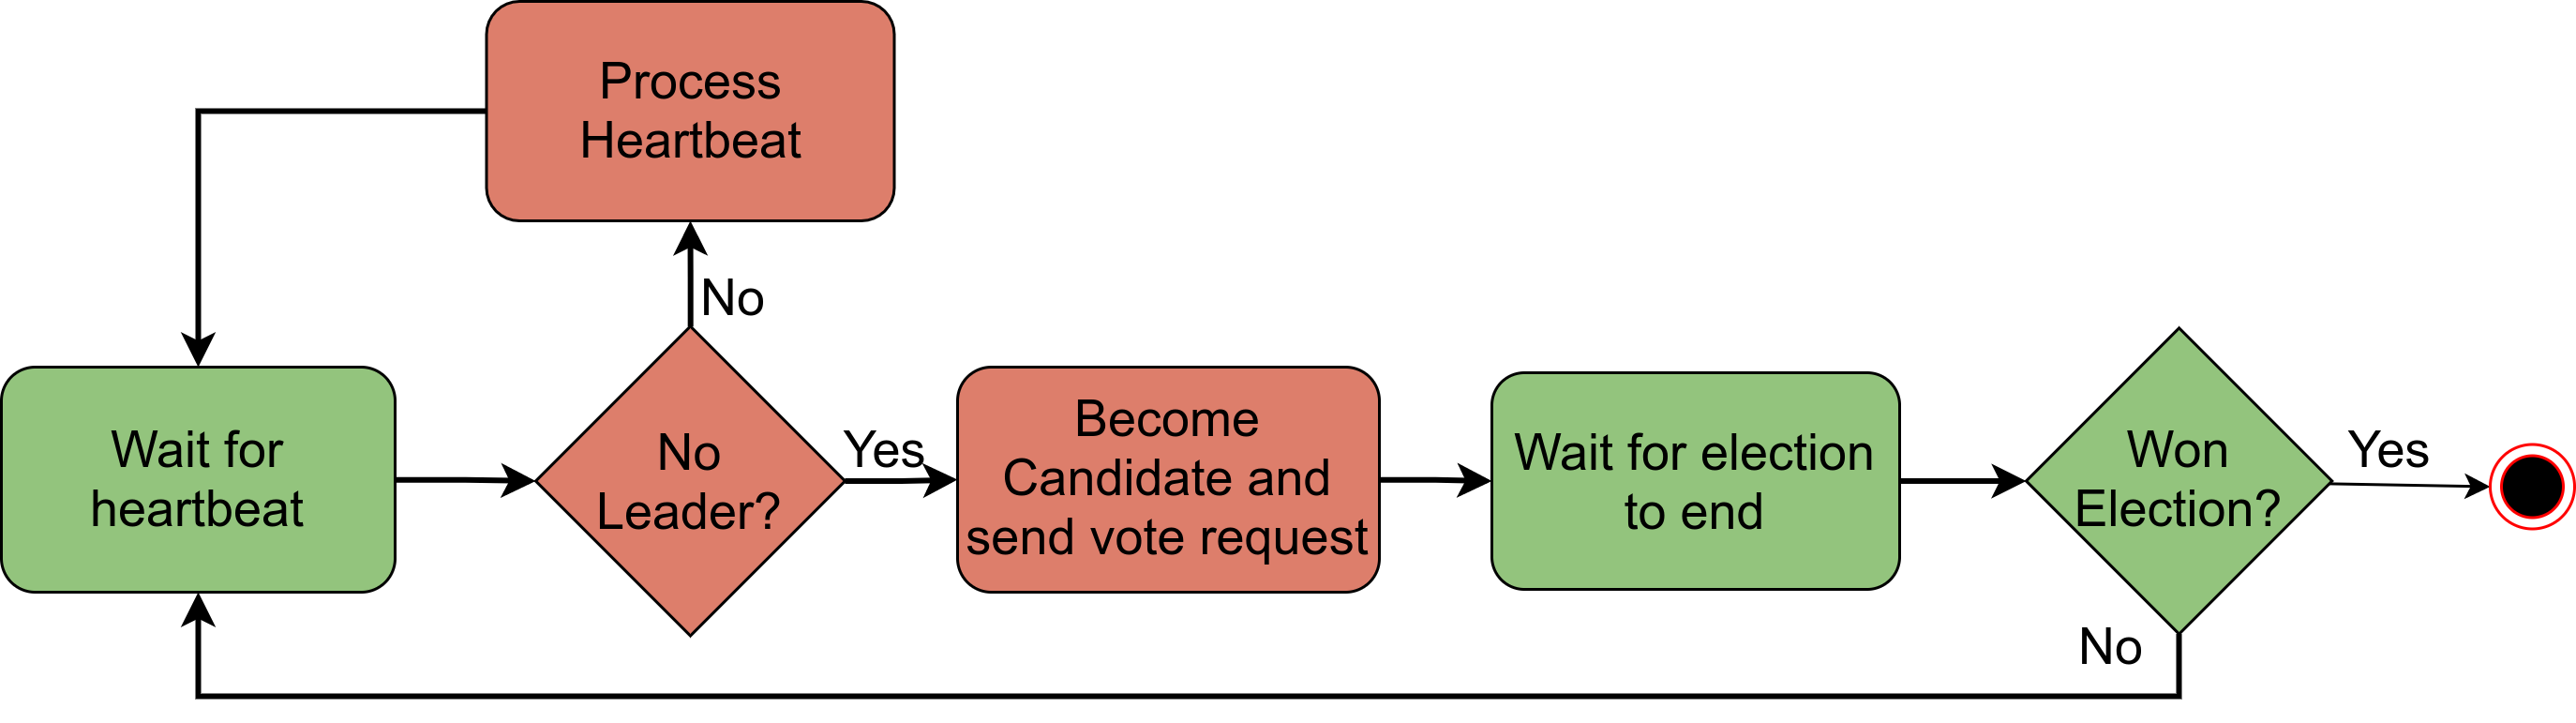
\includegraphics[width=0.9\linewidth]{images/LeaderElectionHeartbeatThread}
	\caption{One part of the leader election process is the monitoring of heartbeat messages. This task is performed by replicas that are in follower state and is used to identify a leader's absence. When no heartbeat messages are received for a certain period of time, a new leader election starts.}
	\label{fig:LeaderElectionHeartbeatThread}
\end{figure}

\begin{figure}[!hb]
	\centering
	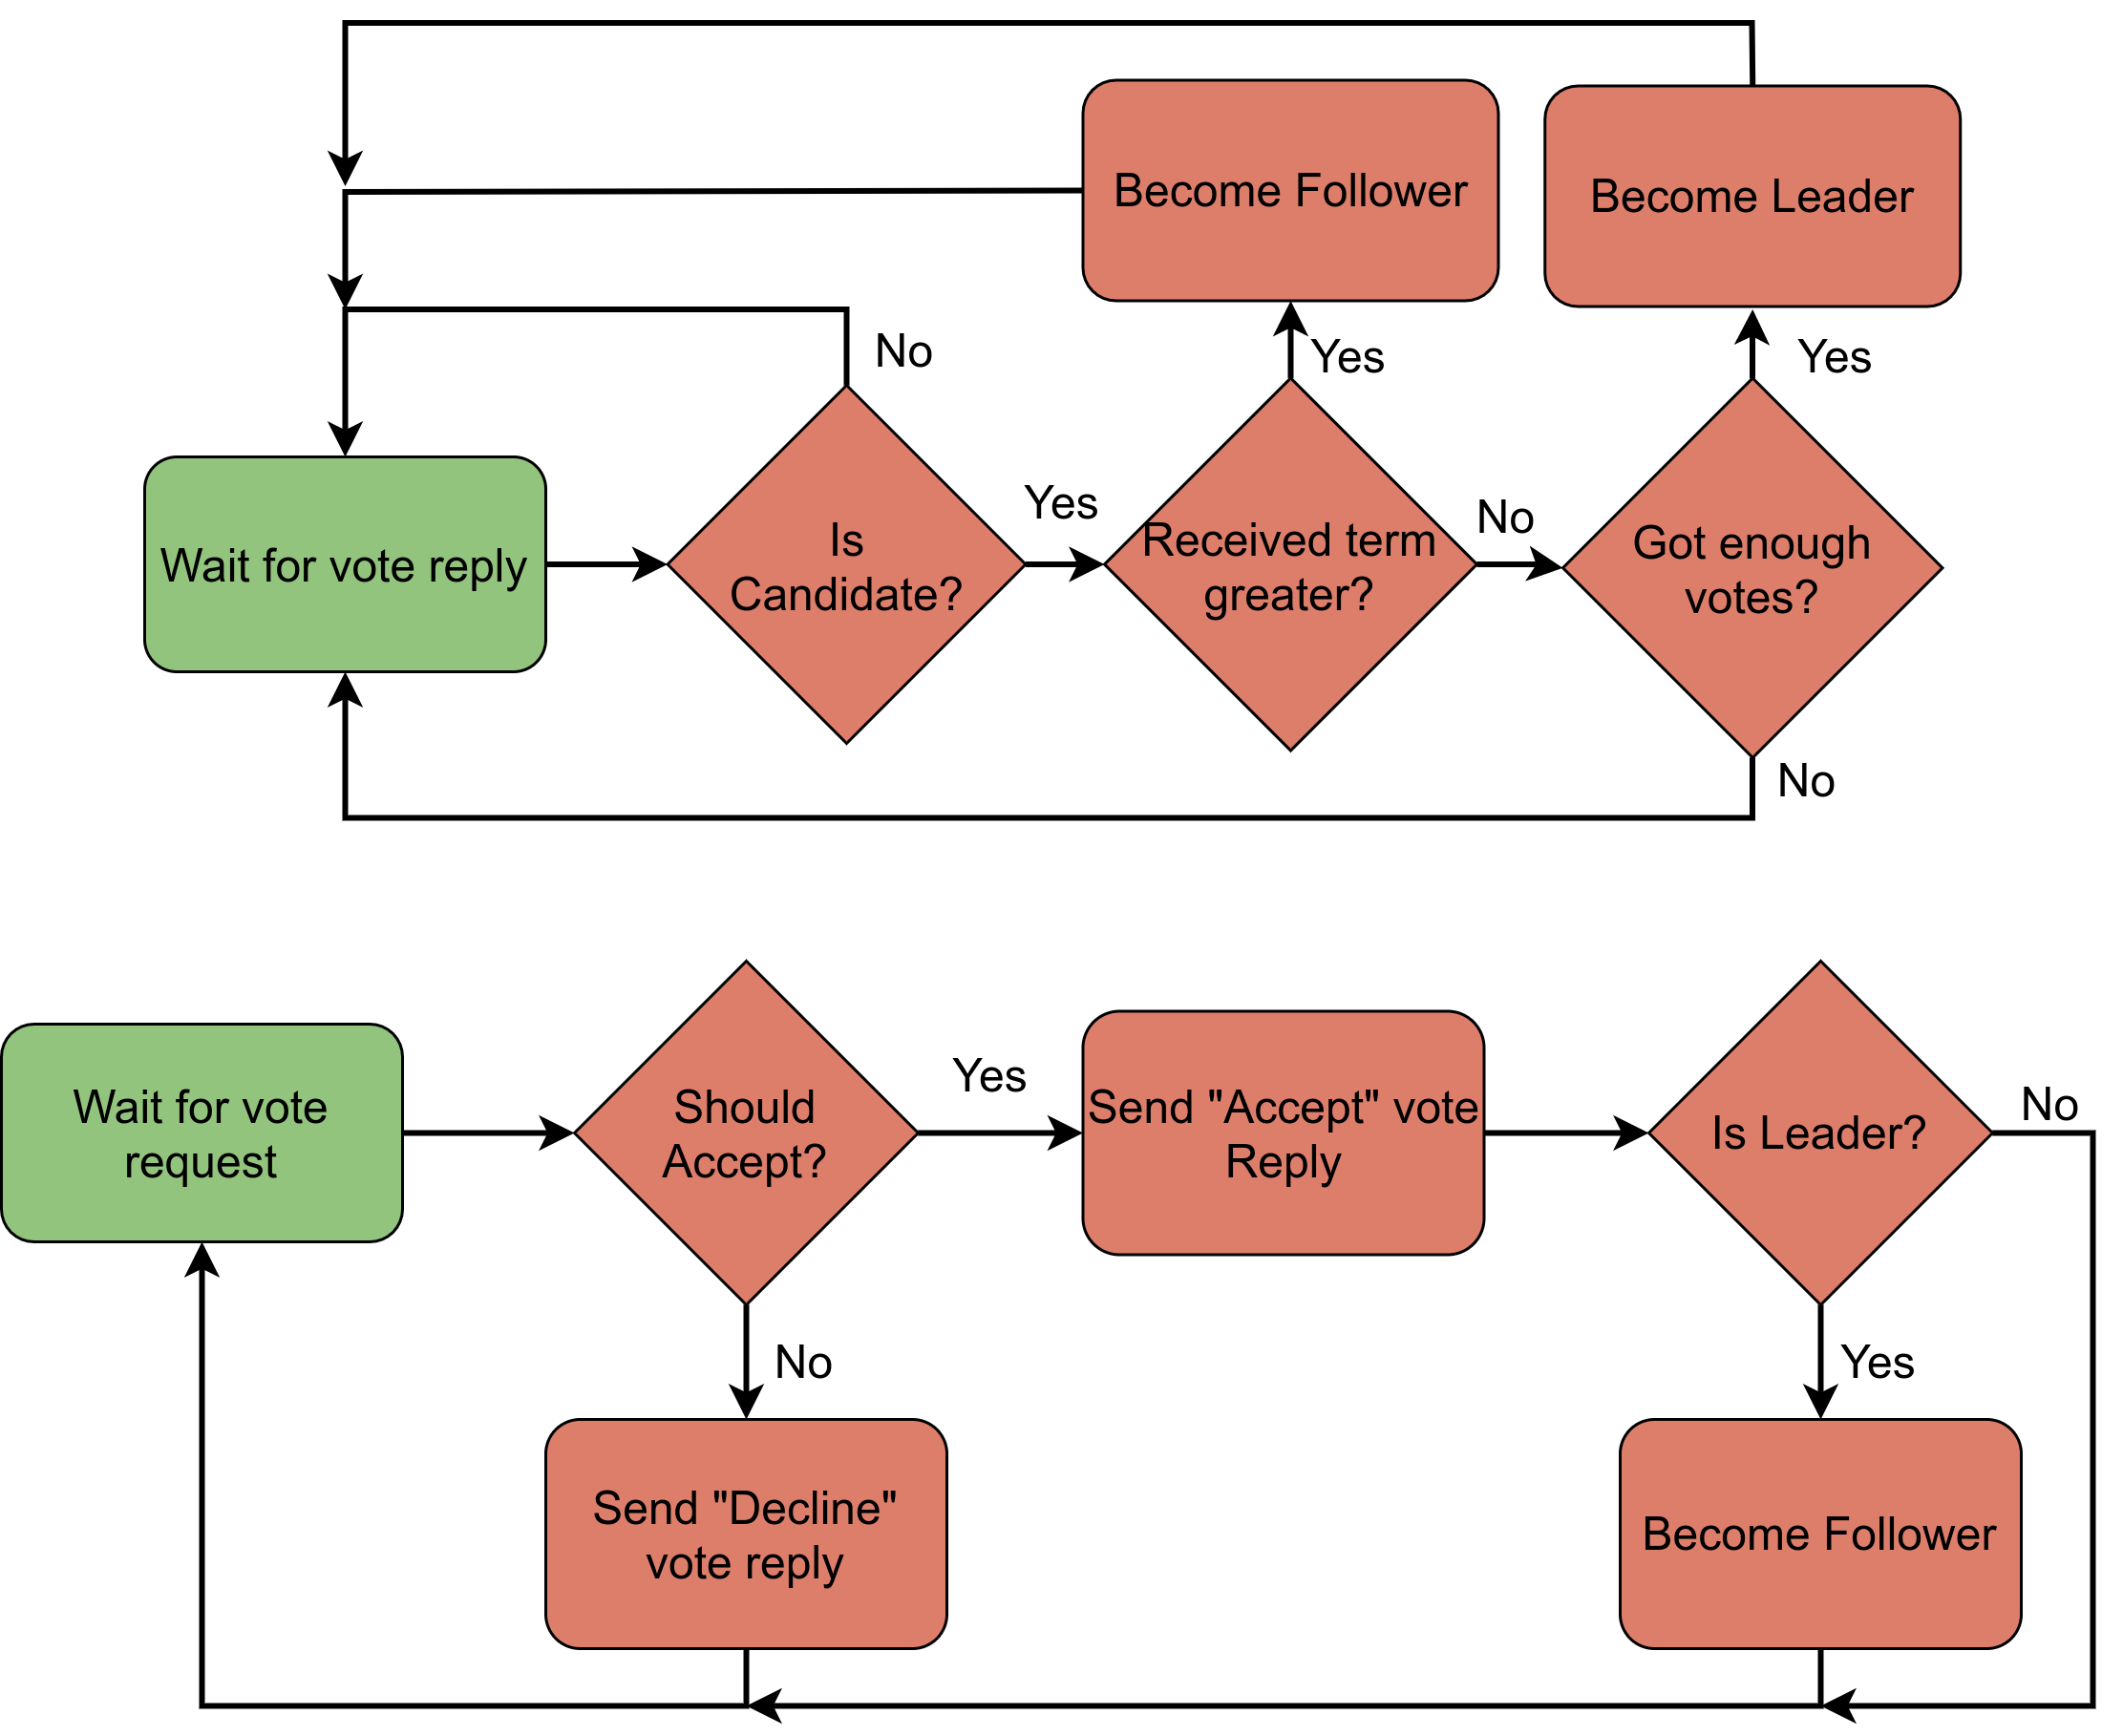
\includegraphics[width=0.9\linewidth]{images/LeaderElectionVoteThread}
	\caption{One part of the leader election process is making and answering vote requests. All replicas are permanently waiting for vote requests. Replicas in candidate state ask the other replicas for their votes and become the new leader after enough votes got accepted.}
	\label{fig:LeaderElectionVoteThread}
\end{figure}


The leader election algorithm is structured into three parts executed on two \abr{OS} threads.
One part is the processing of heartbeat messages in a \texttt{Heartbeat Thread}, as depicted in~\autoref{fig:LeaderElectionHeartbeatThread}.
In the \texttt{Heartbeat Thread}, a follower listens for heartbeat messages and starts a leader election process by sending vote requests when the corresponding timeout expires.
The other two parts, namely answering vote requests and processing replies to vote requests, are handled in another thread and are depicted in~\autoref{fig:LeaderElectionVoteThread}.
Replica-internal race conditions are prevented by utilizing a mutex in order to ensure that its private state - including the replica's \texttt{Raft} role, the current term, and voting information - does not change while answering a message.
Race conditions among replicas are prevented through a history \abr{QOS} policy and a continuously increasing term number.
The history \abr{QOS}-policy ensures that new requests are buffered in a \texttt{DataReader} while another is processed.
This ensures that no request is neglected.
Further, a continuously increasing term number enables the system to detect outdated requests or recognize when the replica itself is outdated.

\subsubsection{Timing Considerations}
\label{subsub:timeConsiderations}

Because each \texttt{WaitSet} in \abr{DDS} can be attached with a timeout, the maximal time that the system is without a leader can be determined.
This is further measured and analyzed in~\autoref{cpt:evaluation}.
There are two timeouts involved in the leader election process, namely the \textit{election timeout} - whereby a missing leader is detected - and the \textit{leader ready timeout}.
An expiring \textit{leader ready timeout} indicates that the system could not elect a new leader for the given term.
This can, for example, happen due to split votes when multiple followers try to become the new leader at the same time or because there are not enough active replicas in the system.
The proposal that \texttt{Raft} makes to reduce the risk of split votes is to use randomized \textit{election timeouts}.
However, this does not prevent split votes from happening at all.
Therefore, in this implementation, the \textit{election timeout} is made directly dependent on the replicas' unique identification number, so that they never try to become a leader at the same time.
Replicas with certain identification numbers are thereby preferred in the leader election process.
However, this approach is not a disadvantage because - due to \abr{DDS}'s global data space - no replica is ever more suitable for becoming the new leader than some other.
Further, a replica with an outdated term number is still excluded from becoming a leader because their vote requests would get declined.

The problem that not enough replicas are active for an election can be solved by specifying the maximum number of consecutive terms that an election is allowed to fail.
Since the \textit{leader ready timeout} states the maximum duration of a failed election, a maximal time that the system is allowed to be without a leader can be specified.
Any replica that recognizes that an election is impossible can then bring the train to a halt.
Altogether, when enough replicas are present in the system and communication is possible without any delays, the system will not be without a leader for the maximum time of $\textit{election timeout} + \textit{leader ready timeout} + \textit{leader election time}$.
\\

Whether a replica writes data onto a topic or reads data from a topic depends on its \texttt{Raft} role.
For example, the leader publishes heartbeat messages while a follower receives the heartbeat messages to detect a missing leader.
Because a replica can become the leader or a follower at any point in time, it cannot be predicted when it transitions from publisher to subscriber or from subscriber to publisher.
This can be a safety hazard because registering a publisher or subscriber can fail and it takes time to register an \abr{DDS} entity to a topic.
Therefore, every replica is set up to simultaneously act as a publisher and subscriber to every topic, with an exception to the \texttt{Input} topic.

However, this also means that each replica receives its own messages.
Therefore, after reading each data sample, the application code must manually verify that the message was not published by the same replica reading the message.
This is done by comparing the receiving replica's identification number with the received \textit{senderID}.
Even though this results in a consistent computational overhead, it increases the implementation's predictability and, thereby, its safety.

\subsection{Decision Making}
\label{subsec:ImpInputProcessing}

\begin{figure}[!hb]
	\centering
	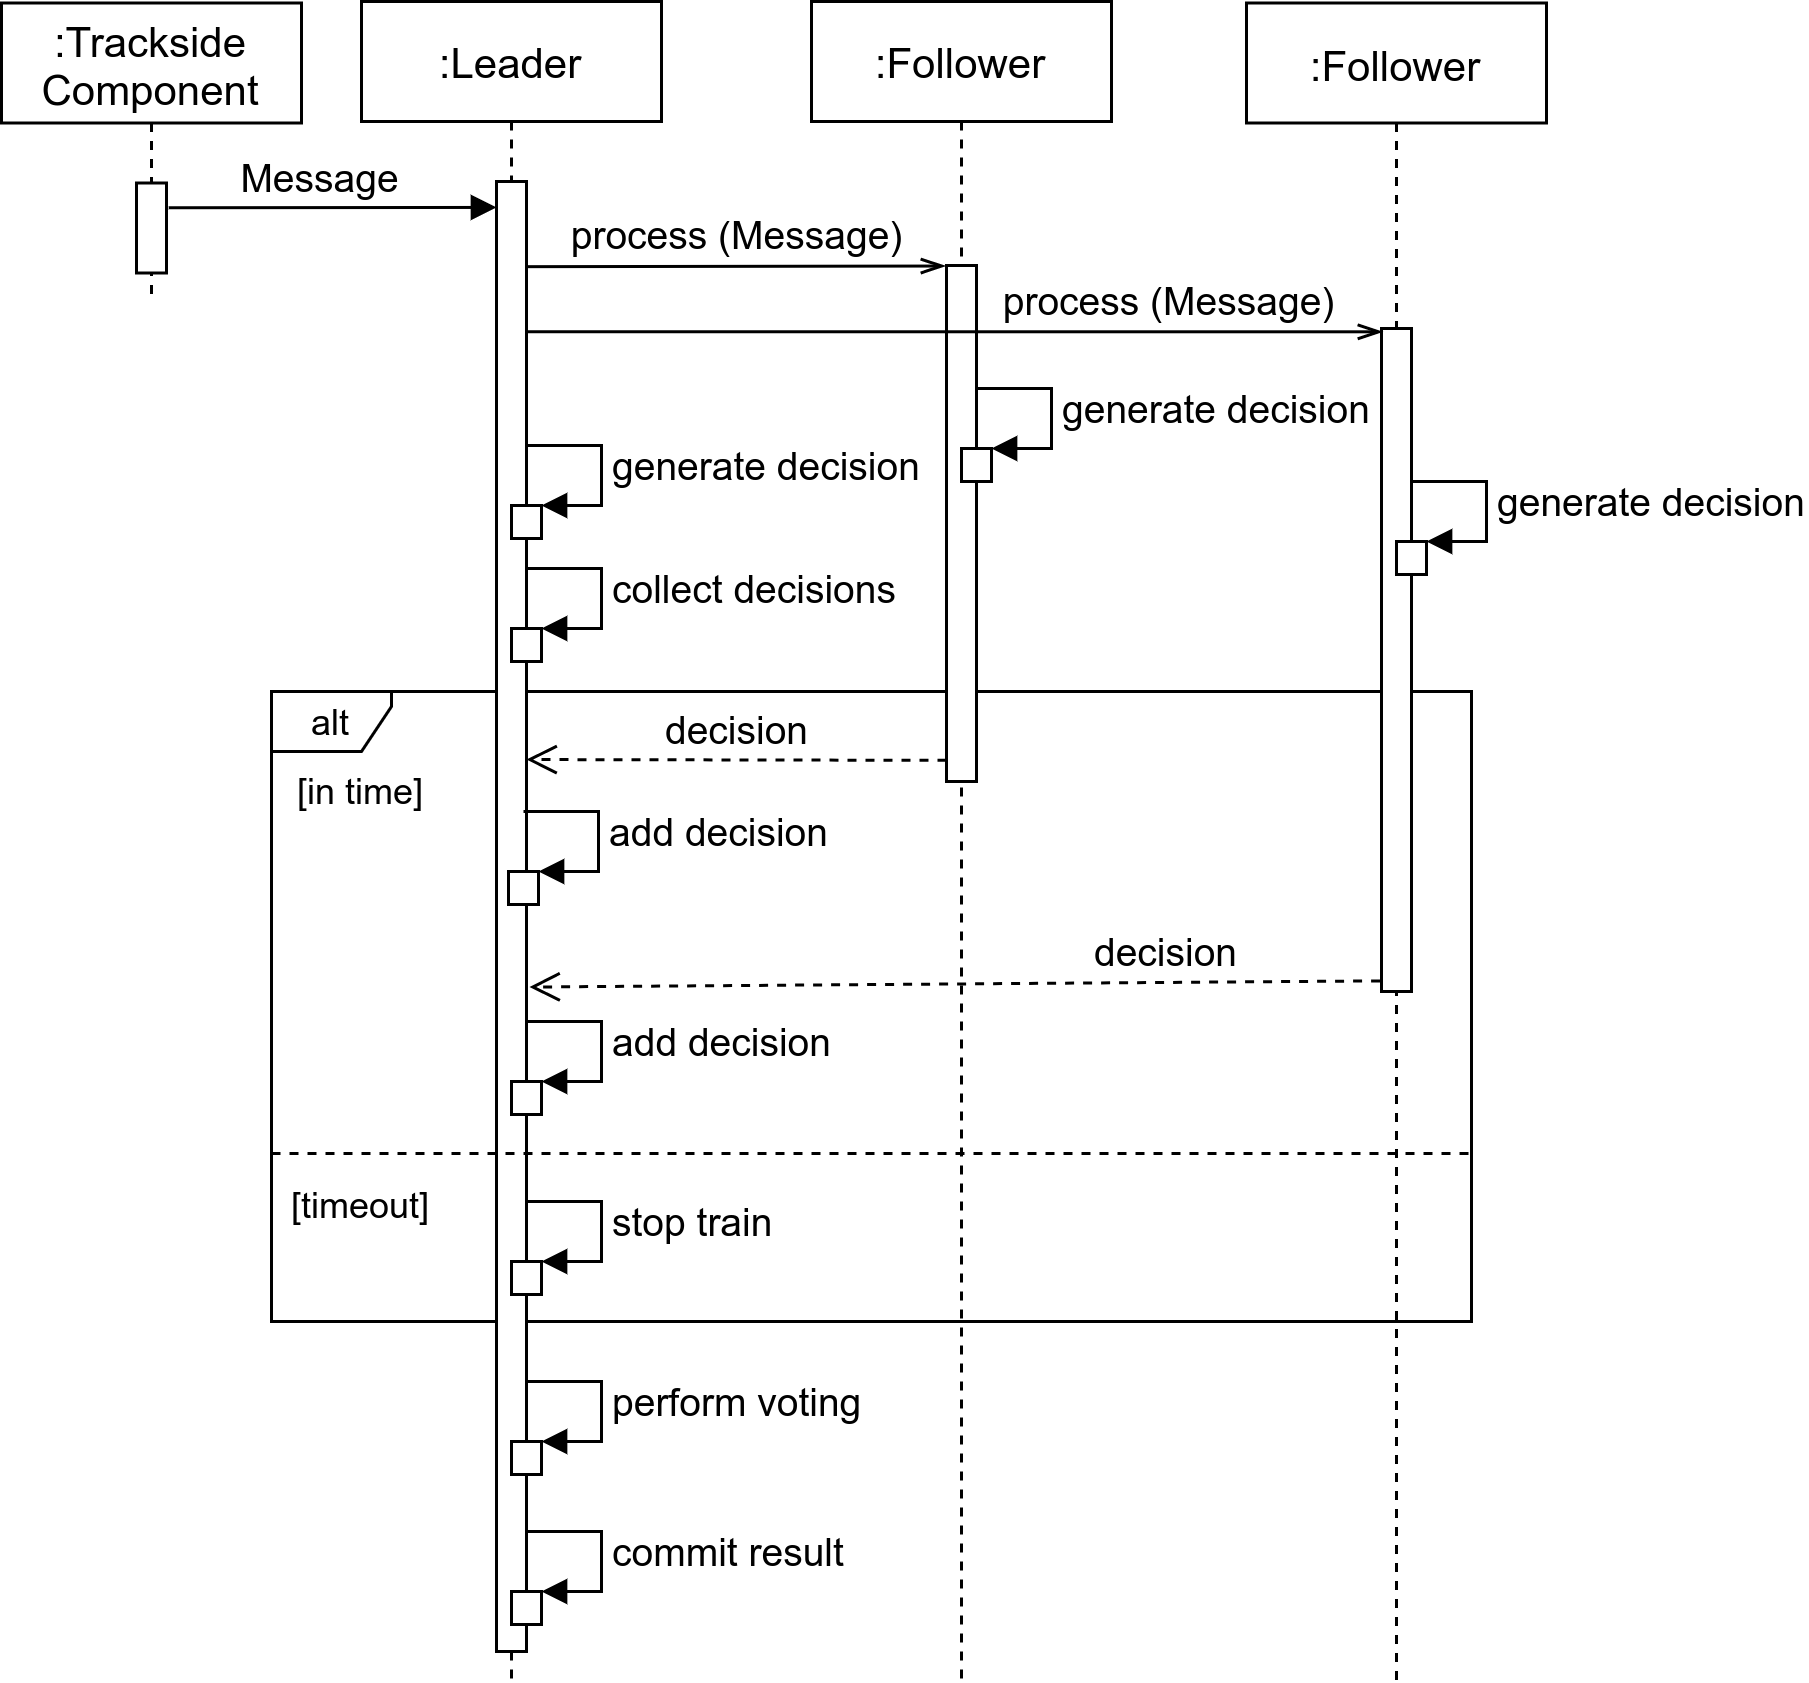
\includegraphics[width=0.8\linewidth]{images/sequence/CollectResults}
	\caption{The leader records input messages from track-side components. Afterward, the leader sends a message with an input reference to each follower in order to request a decision. Then, the leader and each follower process the input and generate a decision based on the input and the global system state. The decisions are collected by the leader that performs a voting when enough decisions are present. Meanwhile, the leader ensures that time constraints are met using timeouts. If there are not enough decisions for voting after the timeout expires, the train must be slowed down.}
	\label{fig:SeqCollectResults}
\end{figure}

Critical input messages, such as balise telegrams, require safety-critical computations and are therefore redundantly processed by the system.
Based on these redundant decisions, the system's leader generates a final system output by performing a majority voting.
A coarse overview of how the redundant computation and voting is performed is shown in~\autoref{fig:SeqCollectResults}.
\\

It is the leader's responsibility to record new inputs, request redundant decisions from the remaining replicas, and generate a voted output based on the redundant decisions.
Therefore, the leader sends a \textit{process} request and a reference to the corresponding input to each follower.
Upon receiving this request, the replicas start to generate a decision for the input.
After sending the request, the leader generates a decision itself and waits for the remaining replicas' decisions.
The leader can perform a majority voting when it received enough redundant decisions after a certain period of time called \textit{processing timeout}.
If there are too few decisions and the system's time constraints are violated, the train must be stopped.
\\

After the leader successfully performed a voting, it commits the final decision.
The commit phase consists of three steps.
First, the system's global state is altered based on the voted decision.
For example, when a linked balise's telegram has been processed, the confidence interval is adjusted to the balise's position.
Second, the leader outputs the voted decision as the system's output.
Third, the corresponding input is marked as processed on the \texttt{Input} topic by disposing of the corresponding \abr{DDS} instance.
This ensures that the next leader will read and process the input if the previous leader is deselected or crashed before committing a result.
\\

Communication between the leader and its followers happens via \abr{DDS} topics.
A \texttt{WaitSet}, attached with a \texttt{ReadCondition}, is used to recognize new messages on the \texttt{Input} topic.
As soon as the leader recognizes a new input message, it sends a \textit{process} request.
The \textit{process} request follows \texttt{Raft}'s log replication approach and is transmitted via the \texttt{AppendEntries} topic.
As soon as a follower receives the \textit{process} instruction, it starts to generate a decision for the referenced input and publish the decision to the \texttt{AppendEntriesReply} topic.
Simultaneously, the leader also generates a decision and waits for follower responses on the \texttt{AppendEntriesReply} topic using a \texttt{WaitSet} and a \texttt{ReadCondition}.

\subsubsection{Safety Considerations}

In order to ensure the train's integrity, every replica's default decision is to brake.
When a balise telegram is received, the train is only allowed to continue its journey if all of the following conditions are met:

\begin{enumerate}
\item The train is currently driving.
\item The balise, to which the received telegram belongs, has been linked.
\item According to the linking information, the balise telegram has been received at the position where the balise should be.
\item According to the braking curve, the train would not reach the current \abr{MA}'s end.
\end{enumerate}

Further, the train's braking curve needs to be periodically monitored independently of incoming balise telegrams.
Therefore, a timeout is attached to the \texttt{Input} topic's \texttt{WaitSet} that expires when no input message is received for a specific period.
Upon expiring, the leader behaves as if an input message has been received.
First, the leader requests redundant decisions whether the train should brake or continue its journey.
Second, the leader calculates a decision itself by calculating the braking curve and comparing it to the current \abr{MA}'s end position.
Third, it waits for results from the remaining replicas and performs a majority voting.
Finally, the voted result is send as a system output.

In the following, both monitoring the braking curve and handling critical inputs is referred to as \textit{input processing}.
\\

When the leader crashed during the small time frame between serving the voted decision as the system's output and marking the corresponding input as processed, an input could be processed twice.
However, it is assumed to be very unlikely that such a situation happens.
In an alternative situation, when the leader would not mark the input as processed, the leader might crash while processing the input, and the input would not be processed at all.
The probability that the leader crashed while processing the input is higher than the probability that it would crash between serving the output and marking the input as processed.
Therefore, the risk of a single input being processed twice is accepted because the alternative is worse and more likely.
\\

For the replicas to generate deterministic and relevant decisions, every replica requires access to the system's most recent global state.
Thus, \abr{DDS} is utilized to manage the system's global state in state topics.
The \texttt{State Manager} component, that is responsible for managing the global state, is described in~\autoref{sec:stateManager}.

Because only the leader can change the global state, updates must be sent to all replicas.
Hence, redundant decisions can be based on different state information and thereby affect the system's safety.
A possible way to reduce the chance of such situations is to repeat the input processing when the leader's decision was outnumbered in the voting.
However, only if the repetition would not jeopardize any time constraints.

\subsubsection{Timing Considerations}

After the leader sent a decision request to every other replica and generated a decision itself, it waits for responses to continue with voting.
Since the system consists of independent replicas, it is impossible to predict how long it will take the other replicas to generate a decision.
In order to prevent the voting process from being deferred indefinitely, a timeout is attached to the \texttt{WaitSet} for the \texttt{AppendEntriesReply} topic.
Consequently, two situations are possible while the leader waits for responses on the \texttt{AppendEntriesReply} topic.
First, the leader receives a response from every replica before the timeout expires.
Second, the timeout expires before a response from every replica has been received.
In the first situation, voting is possible without any problems.
In the second situation, the leader can only continue when a response from more than half of the replicas in the system have been received.
If the leader received an even number of decisions, split votes in the voting process are possible.
In case of split votes, the most restrictive one has to be chosen.
Receiving too few decisions is a safety risk and the leader must stop the train.
\\

In addition, a leader could repeatedly crash while processing an input.
Thereby, the system would not be able to generate an output for a critical input.
The presented system cannot cope with such a situation because it would require a distributed timeout that is not possible for an asynchronous system~\cite{FLPProblemConsensus}.
It could be solved by an external instance that recognizes incoming inputs and stops the train when it is not notified that an output has been generated.
In practice, the antenna unit could perform this task by applying a counter and being connected to the on-board unit's output line.

\section{System Recovery}

The failure of system components reduces the system's reliability (ref.~\autoref{sec:techniquesSafetyReliability}).
This section describes methods by which the system can recover from the failure of individual components and thus retain its reliability.
Such procedures are based on the concepts of error detection, location, and recovery.
\\

First, the implementation of hot standby redundancy using DDS concepts is described.
Afterward, it is explained how the hardware watchdog of the \textit{Revolutions Pis} can be used to increase reliability - as proposed by Sakic and Kellerer~\cite{SakicTimeInConsensus}.

\subsection{Hot Standby}
\label{sec:HotStandby}

\begin{figure}[!ht]
	\centering
	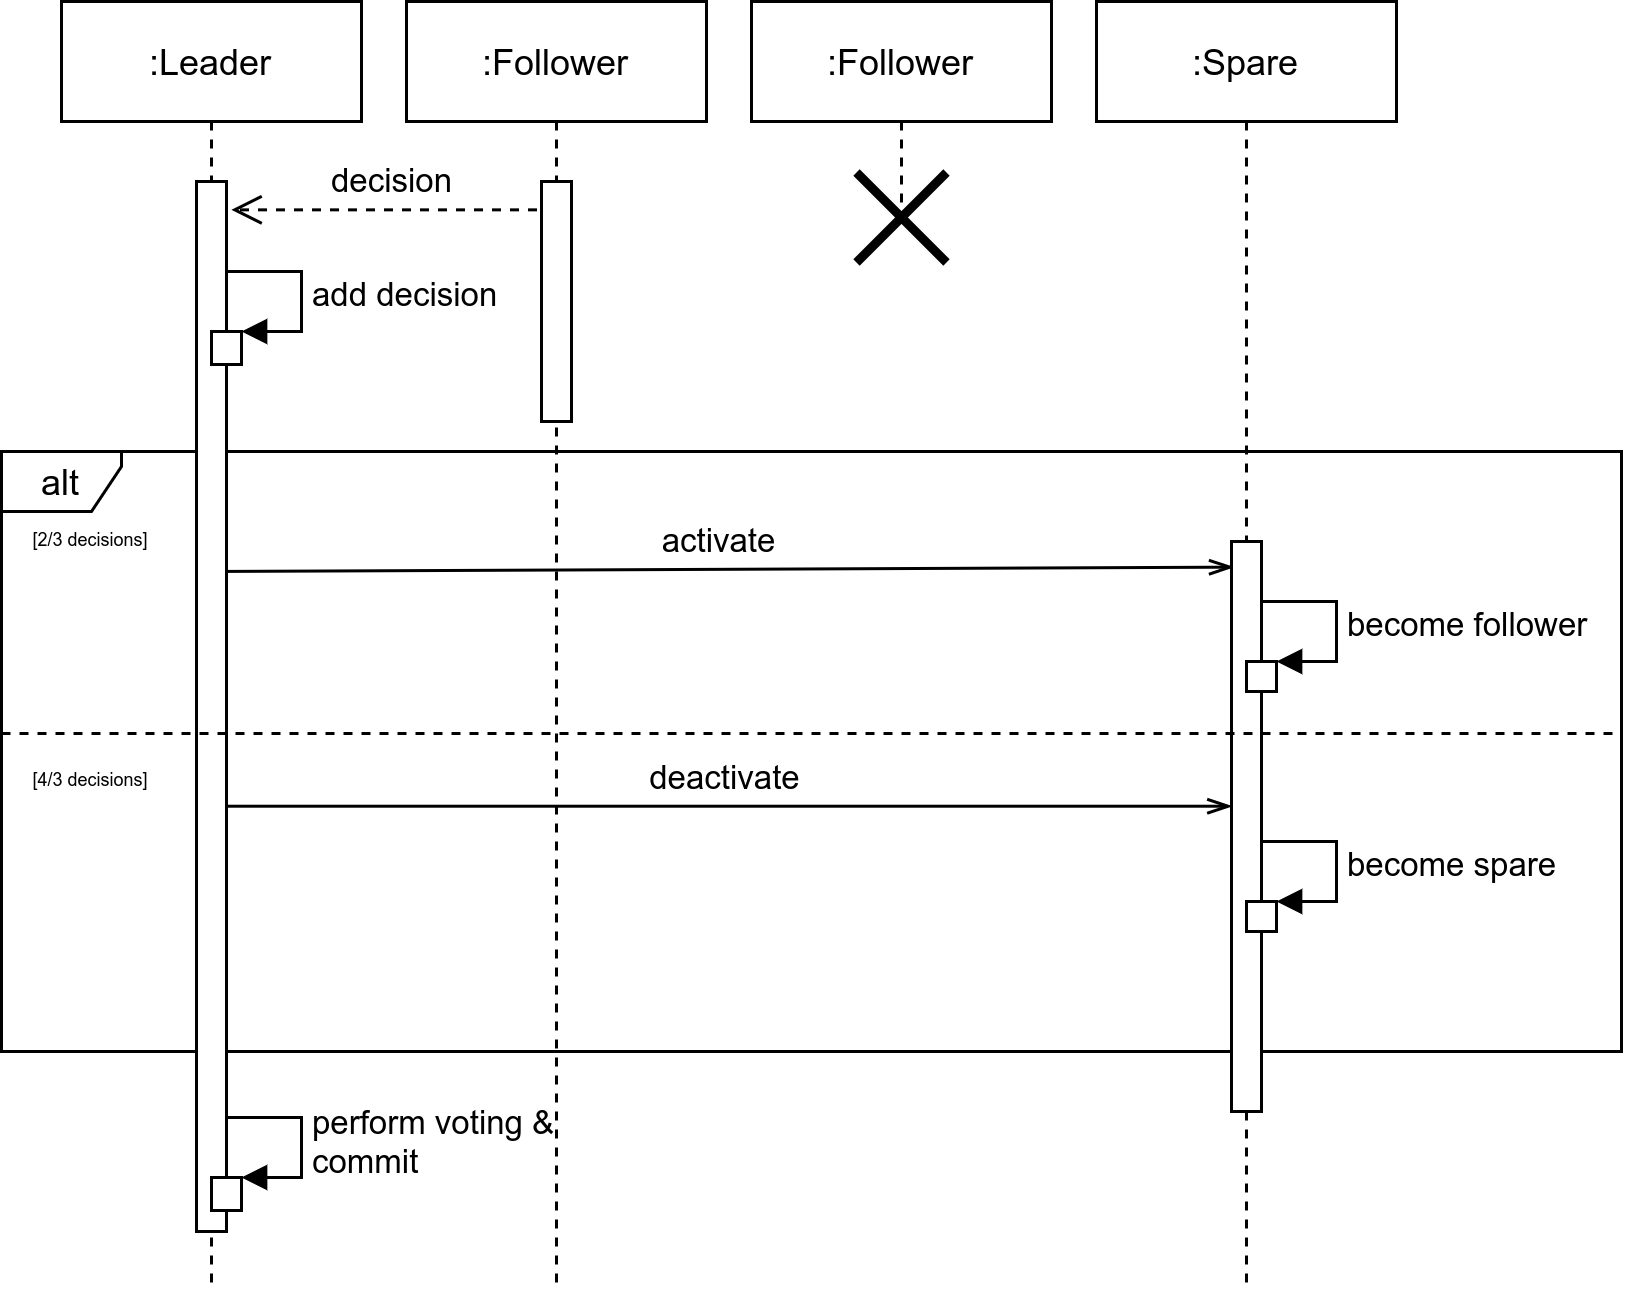
\includegraphics[width=0.75\linewidth]{images/sequence/ActivateSpare}
	\caption{When the leader, after reading an input message and instructing its followers to process the input, receives too few decisions after a certain time, it activates the spare replica. When the leader receives more decisions than necessary, the spare component is deactivated again.}
	\label{fig:SeqActivateSpare}
\end{figure}

Active hardware redundancy facilitates systems to recover from individual component failures.
An algorithm for adding a spare component as a hot standby is depicted in~\autoref{fig:TMRWithSparesDDS}.
If the leader receives too few decisions when processing an input, it assumes that any non-responsive replica has crashed.
Thereupon, the leader activates the spare by publishing a message to a \abr{DDS} event topic called \texttt{ActivateSpare}.
If the replica that was presumed crashed responds again, the spare can be deactivated again by publishing a corresponding message to the \texttt{ActivateSpare} topic.
\\

For creating a hot standby, a component must be initialized in spare mode.
Spare mode implies that the component is initialized as any other component but additionally subscribes to the \texttt{ActivateSpare} topic.
Further, a spare utilizes a \texttt{WaitSet} to wait for any activate message.
\\

Unlike the other replicas, a spare component can only be in \texttt{spare} or \texttt{follower} mode and is excluded from becoming the leader, as well as from voting for other leaders in the leader election process.
This is because a spare component can be activated or deactivated at any time.
Upon being activated, a spare component participates in the input processing process by responding to leader requests.
\\

Although only a single spare component is currently supported, multiple spares can be added by introducing a \texttt{spareID} field to \texttt{ActivateSpare}.

\subsection{Watchdog}

A watchdog is an important safety feature and proposed by Sakic and Kellerer~\cite{SakicTimeInConsensus} to increase a system's probability to respond when a component failed.
\textit{Revolution Pi Connects} install a configurable hardware watchdog in the form of a watchdog timer on a dedicated hardware chip.
The timer must be manually and periodically reset.
When it is not reset, the timer expires and the corresponding \abr{PLC} restarts.
This allows the watchdog to restart a replica when the on-board unit software stops responding.
\\

In order to take advantage of the hardware watchdog, the heartbeat mechanism used for the consensus algorithm is exploited.
Each time the leader sends a heartbeat, it also resets the watchdog timer.
For followers, the watchdog timer is reset upon receiving a heartbeat message.

On the one hand, this increases the system's reliability because certain exceptions and faults, such as memory corruptions, that result in a stopped software can be repaired by restarting the system.
On the other hand, an appropriate watchdog timeout must be small enough to restart a faulty component as soon as possible but long enough not to trigger false positives.
Since resetting the timer is bound to the heartbeat mechanisms, the maximum time that the system can be without a leader needs to be known.
This is analyzed in~\autoref{subsec:LeaderElectionEval} and marks the watchdog timer's lower limit.


\iffalse






\begin{figure}[!hb]
	\centering
	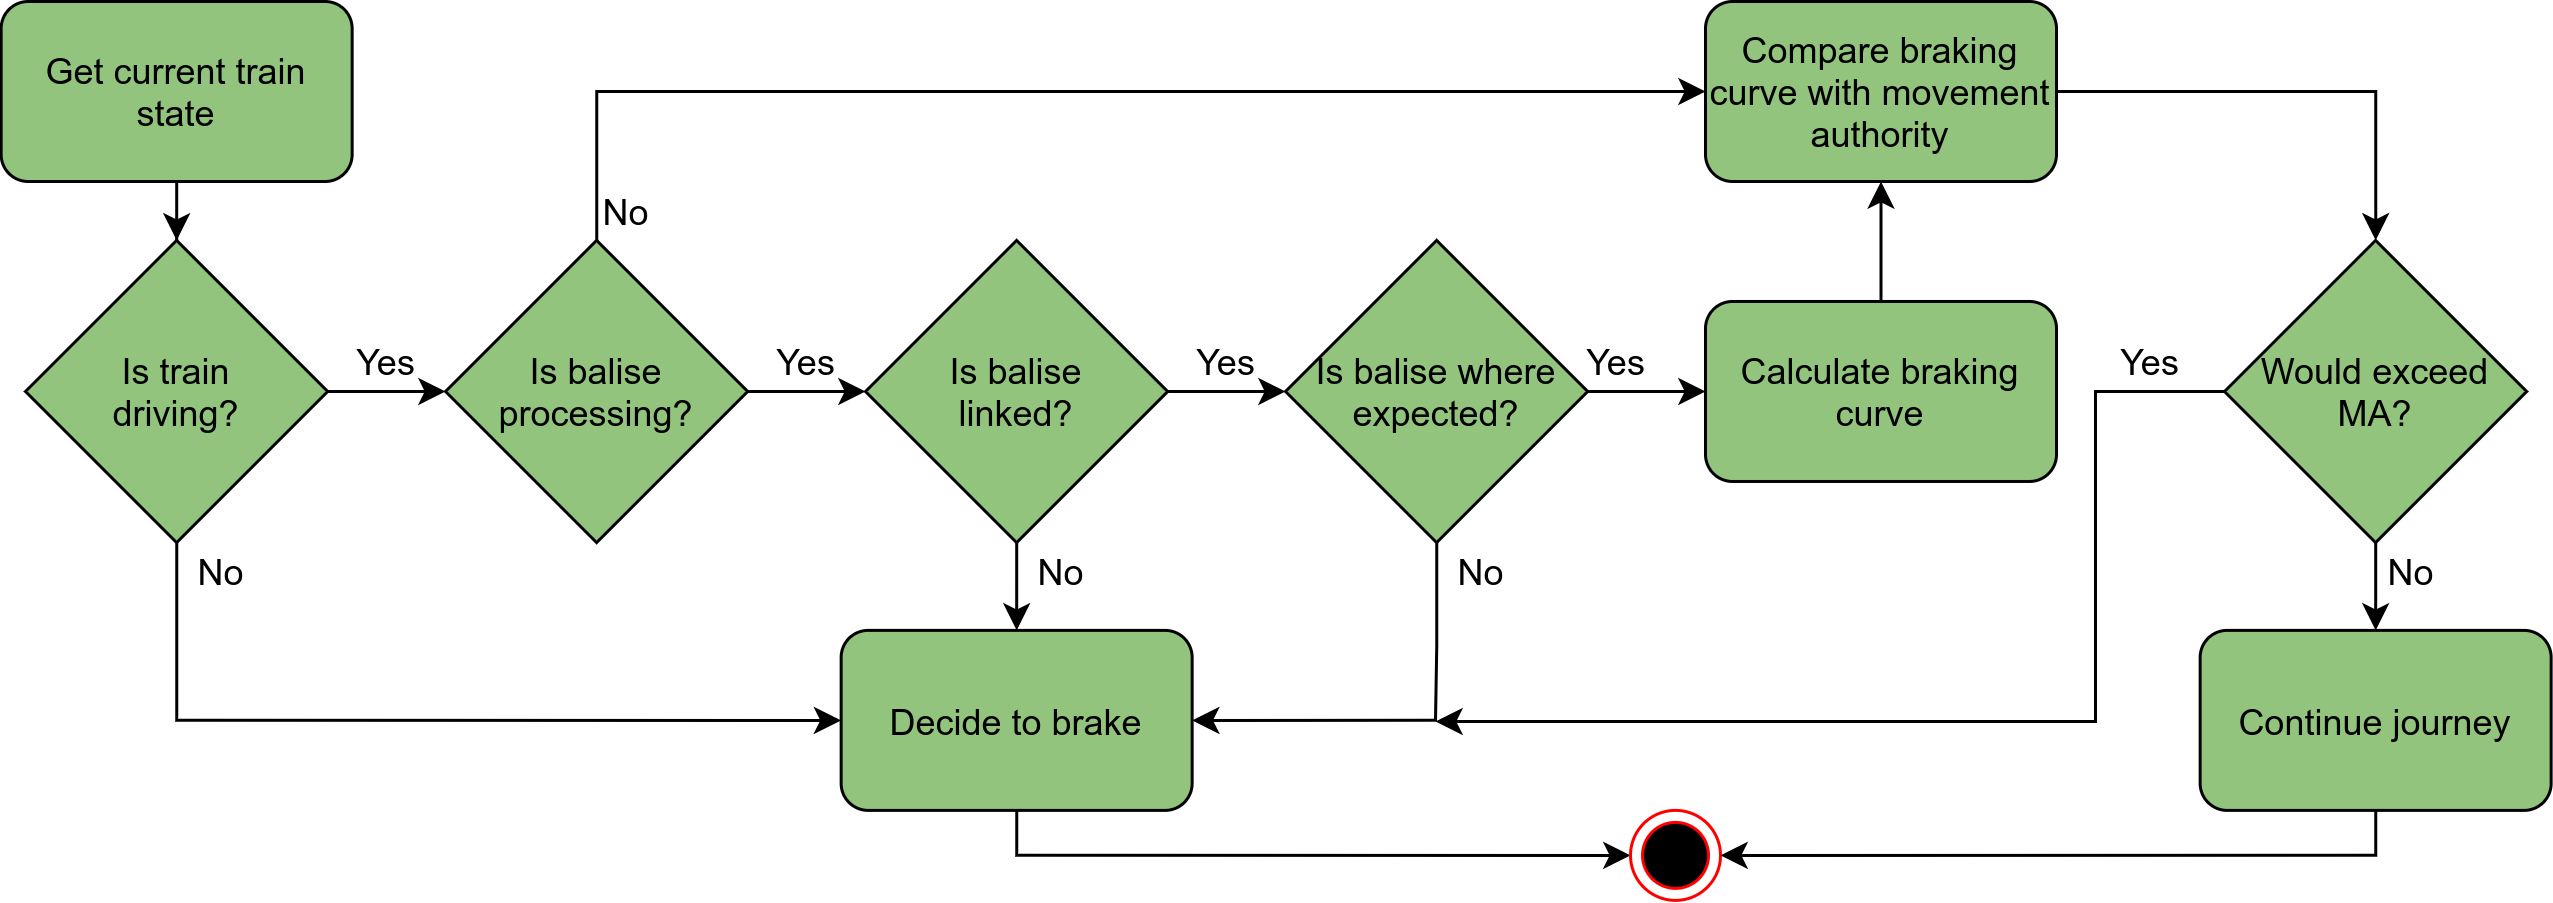
\includegraphics[width=0.75\linewidth]{images/DecisionMaking}
	\caption{To decide whether the train should brake or can continue its journey, this algorithm is executed. When the train is not driving, it should brake. IF a balise telegram is evaluated, it is checked whether the balise is linked and whether the calculated train position corresponds with the balise's expected position. Finally, the train's braking curve is calculated and it is checked, whether the train would reach the current \glsentryfull{MA}'s end position when it would brake in this moment. Only if everything goes as planned may the train continue its journey.}
	\label{fig:DecisionMaking}
\end{figure}

\begin{algorithm}[H]\caption{TODO.}\label{algo:DecisionMaking}
\SetKwData{MA}{\textit{\abr{MA}}}
\SetKwData{LinkedBalises}{\textit{linked balises}}
\SetKwData{TrainState}{\textit{train state}}
\SetKwInOut{Input}{input}
\SetKwInOut{Output}{output}

\Input{A balise telegram to process, the current \MA, the set of \LinkedBalises, and the \TrainState}
\Output{Decision to brake or continue the journey}
\BlankLine

\If{The train is not driving}{
brake\;
return\;
}
\If{processed balise is not linked}{
brake\;
return\;
}
\If{processed balise's position not in confidence interval}{
brake\;
return\;
}
calculateBrakingCurve()\;
\If{Train would reach end of \MA when braking now}{
brake\;
return\;
}
continue journey\;
return\;
\end{algorithm}





\lstset{language=C}
\begin{lstlisting}[caption={\abr{IDL} definition for the \texttt{AppendEntries} topic. The \texttt{term} variable represents the latest term that the replica has seen, while the \texttt{senderID} encodes which replica sent this message. With \texttt{entries}, a payload can be send via the topic. This is used by a leader for instructing its followers to process certain data. The \texttt{entries} field is left empty for heartbeat messages.}, label=code:appendEntries]
struct AppendEntries {
    long term;
    long senderID;
    sequence<Entry> entries;
};
#pragma keylist AppendEntries term
\end{lstlisting}

\begin{lstlisting}[caption={\abr{IDL} definition for the \texttt{RequestVote} topic. The \texttt{term} variable represents the candidate's term, while \texttt{candidateID} encodes the candidate that requested the vote.}, label=code:requestVote]
struct RequestVote {
    long term;
    long candidateID;
};
#pragma keylist RequestVote
\end{lstlisting}

\begin{lstlisting}[caption={\abr{IDL} definition for the \texttt{RequestVoteReply} topic. The \texttt{term} encodes the sender's term for the candidate to update itself. \texttt{voteGranted} shows whether the replica granted the vote request for the given term. The \texttt{candidateID} and \texttt{senderID} are used to identify which replica granted the vote for which replica respectively.}, label=code:requestVoteReply]
struct RequestVoteReply {
    long senderID;
    long term;
    long candidateID;
    long voteGranted;
};
#pragma keylist RequestVoteReply
\end{lstlisting}



\begin{lstlisting}[caption={\abr{IDL} definition for the \texttt{LinkedBalises} topic. Each linked balise has an unique identifier and a position that is communicated to the system by the \abr{RBC}.}, label=code:linkedBalises]
struct LinkedBalises {
    short ID;
    long position;
};
#pragma keylist LinkedBalises ID
\end{lstlisting}

\begin{lstlisting}[caption={\abr{IDL} definition for the \texttt{MovementAuthority} topic. The \texttt{start\_position} encodes where the \abr{MA} starts and the \texttt{end\_position} encodes until where it is valid.}, label=code:movementAuthority]
struct MovementAuthority {
    long start_position;
    long end_position;
};
#pragma keylist MovementAuthority
\end{lstlisting}

\begin{lstlisting}[caption={\abr{IDL} definition for the \texttt{TrainState} topic. The train's state consists of a current position and a current speed. Due to inaccuracies of the position sensors, a train's position cannot be determined exactly. Therefore, a confidence interval is maintained that defines an area where the train certainly is. This area is bounded by \texttt{max\_position} and \texttt{min\_position}. With \texttt{is\_driving} it is encoded whether the virtual train drives or stands still. The \texttt{lastUpdateTime} variable is used to simulate the train's position based on its speed.}, label=code:trainState]
struct TrainState {
    double position;
    double max_position;
    double min_position;
    double speed;
    boolean is_driving;
    unsigned long long lastUpdateTime;
};
#pragma keylist TrainState
\end{lstlisting}

\begin{lstlisting}[caption={\abr{IDL} definition for the \texttt{ActivateSpare} topic. This topic is used to activate or deactivate spare replicas. The \texttt{term} field encodes the term in which the activate or deactivate call has been made and \texttt{activate} gets interpreted as a boolean that encodes whether the spare should be activated or deactivated.}, label=code:activateSpare]
struct ActivateSpare {
    long term;
    long activate;
};
#pragma keylist ActivateSpare
\end{lstlisting}

\fi
